\documentclass{article}[12pt]
\usepackage{color}
\usepackage[normalem]{ulem}
\usepackage{times}
\usepackage{fullpage}
\usepackage{amsmath}
\usepackage{amssymb}
\usepackage{tikz}
\usepackage{graphicx}
\def \R {\mathbb R}
\def \imp {\Longrightarrow}
\def \eps {\varepsilon}
\def \Inf {{\sf Inf}}
\newenvironment{proof}{{\bf Proof.  }}{\hfill$\Box$}
\newtheorem{theorem}{Theorem}[section]
\newtheorem{definition}{Definition}[section]
\newtheorem{corollary}{Corollary}[section]
\newtheorem{lemma}{Lemma}[section]
\newtheorem{claim}{Claim}[section]
\setlength {\parskip}{2pt}
\setlength{\parindent}{0pt}

\newcommand{\headings}[4]{\noindent {\bf Assignment 1 CME241} \hfill {{\bf Author:} Nicolas Sanchez} \\
{} \hfill {{\bf Due Date:} #2} \\

\rule[0.1in]{\textwidth}{0.025in}
}

\newcommand{\klnote}[1]{{\color{red} #1}}
\newcommand{\klsout}[1]{{\color{red} \sout{#1}}}

\begin{document}

\headings{\#1}{Tuesday, October 8, 10:30am}\section{} 



\section{Snakes and Ladders}

{\em Draw} DFAs for the following languages. (Please don't give 5-tuples!) Give brief justification for your answers. For full credit, use the smallest number of states that you possibly can. Please draw neatly or use the TikZ package (see Piazza for TikZ pointers).

\begin{itemize}
\item[(a)] The state space for this game can be succintly represented by one integer between 1 and 100 representing the tile where the player is located at time $t$. Formally
\begin{align*}
S_t \in \mathbf{S}& =\{1,\ldots 100\}\\
\mathbf{T}& = \{100\}
\end{align*} 
\item[(b)] The transition probabilities follow the dice rolls as well as snake ladder combinations with some exceptions for the last 6 tiles of the game. Formally we have:
\begin{align*}
P(i,m[j]) =  \begin{cases} 0 \text{ if $j\leq i$ or $j> i+6$}\\ \frac{1}{6} \text{ if $j<100$} \\ \frac{(i+7)-100}{6} \end{cases}\\
\end{align*} 
where $m[j]$ maps $j$ to the end of the snake if $j$ is the start of a snake, the end of the ladder if $j$ is the start of a ladder or itself in all other cases.\\


\item[(c)]  If every pair of state/transition is rewarded by 1 without any discount, then the cumulative reward of a given path will be the number of rolls. This is implemented in the code and a snippet output of the code with a sample trace and the expected number of rolls (calculated by finding the value of state 1) of roughly 36.6 rolls is included below.



\begin{figure}
  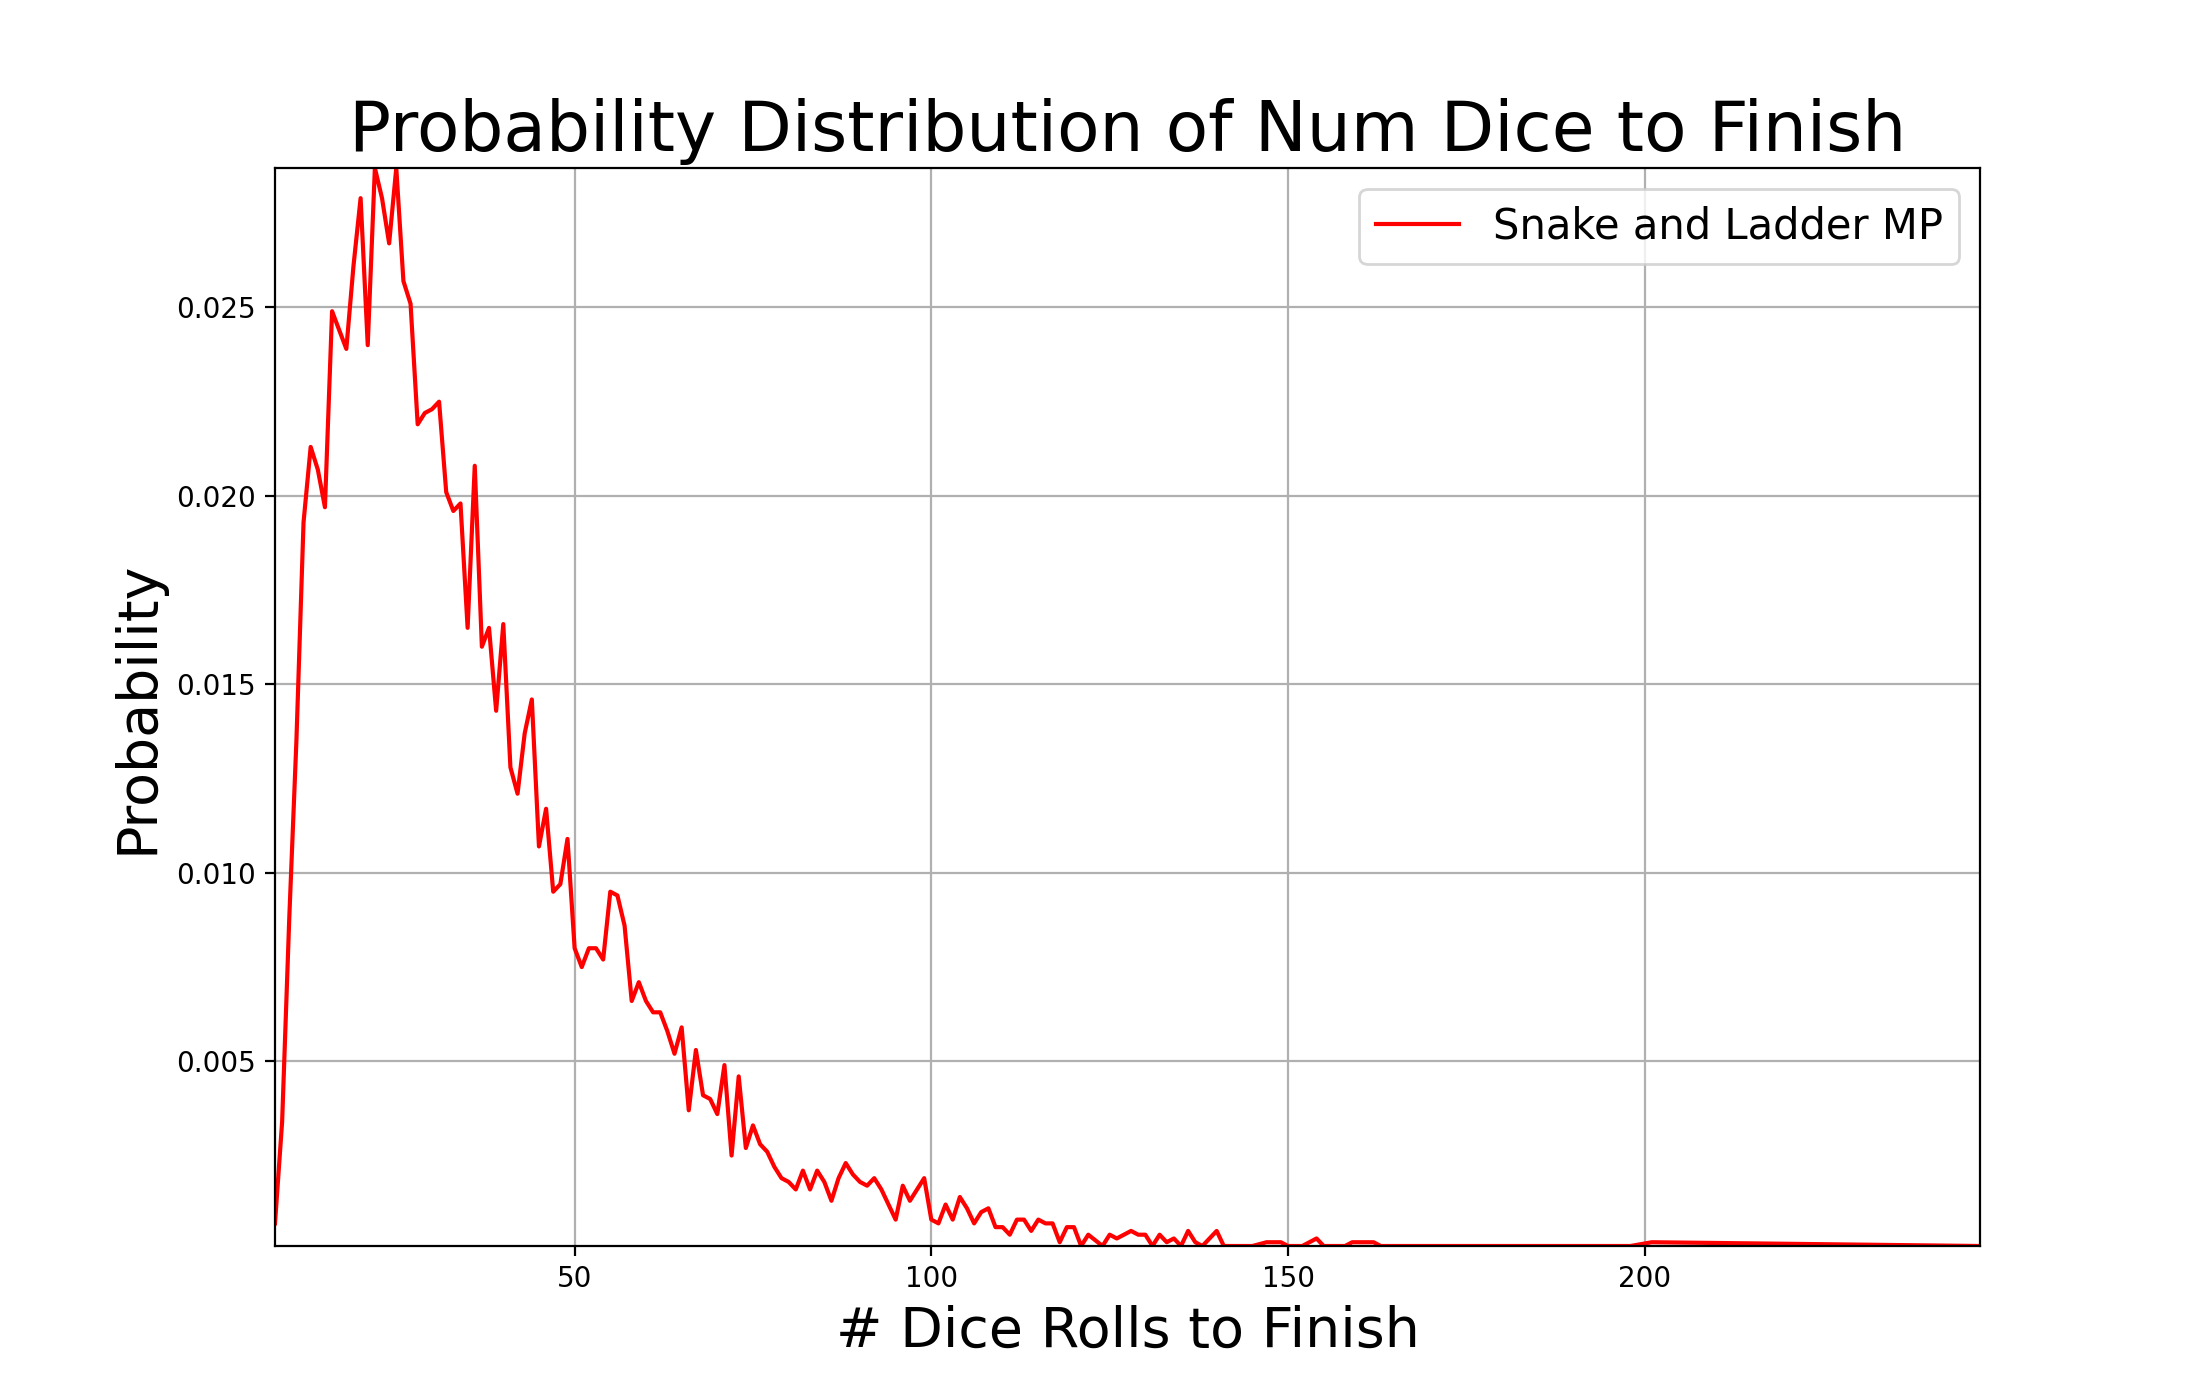
\includegraphics[width=\linewidth]{probs_num_rolls_finish.png}
  \caption{Roll Distribution for Snakes and Ladders}
  \label{fig:rollDist}
\end{figure}

\begin{figure}
  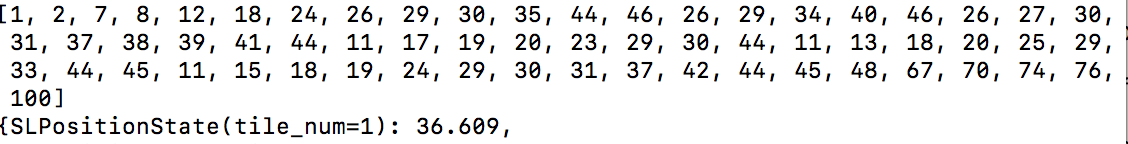
\includegraphics[width=\linewidth]{curl.png}
  \caption{Example Code Output for Snakes and Ladders}
  \label{fig:term_out}
\end{figure}
\end{itemize}
\section{Frog Puzzle}

We can think of the state here to be the number of the leaf that the number is on. We suppose here that there are $n$ such leaves. We can then define the transition probabilities at each leaf $i$:

\begin{align*}
P(i,j) =  \begin{cases} 0 \text{ if $j\leq i$}\\ \frac{1}{n-i} \text{ if $j>i$} \end{cases}\\
\end{align*} 

Using the same trick that we did in Snakes and Ladders where we define the reward to be 1 for every state and transition and a discount of 1 to get the cumulative reward of a pass being the number of jumps. Thus we can get an analytical solution for this problem by taking the first element of the value vector:
$$ v = (I_n - P)^{-1}$$

Given the structure of the transition probability we know by the bellman equation that the value of any state $i$ depends only on subsequent states $j$ with $j>i$. Specifically we get an induction relation with:
\begin{align*}
v[n] &= 0\\
v[i] &= 1 + \frac{1}{n-i}\sum_{j = i+1}^n v[j]
\end{align*}


\section{Extended Stock Price}

We extended the Stock Price MRP as requested and tested with simple function that adds the difference between the stock price and reversion level at every step, crudely representing the final returns on a strategy that always sold levels above the reversion level. This could be somewhat relevant for a party trading futures oscillation while having access to the underlying deliverable at a realisable L level. This does not take into account mark to market or inventory shortage/balance sheet shortages but serves to test the function.

Below is the price evolution and the cumulative return.


\begin{figure}
  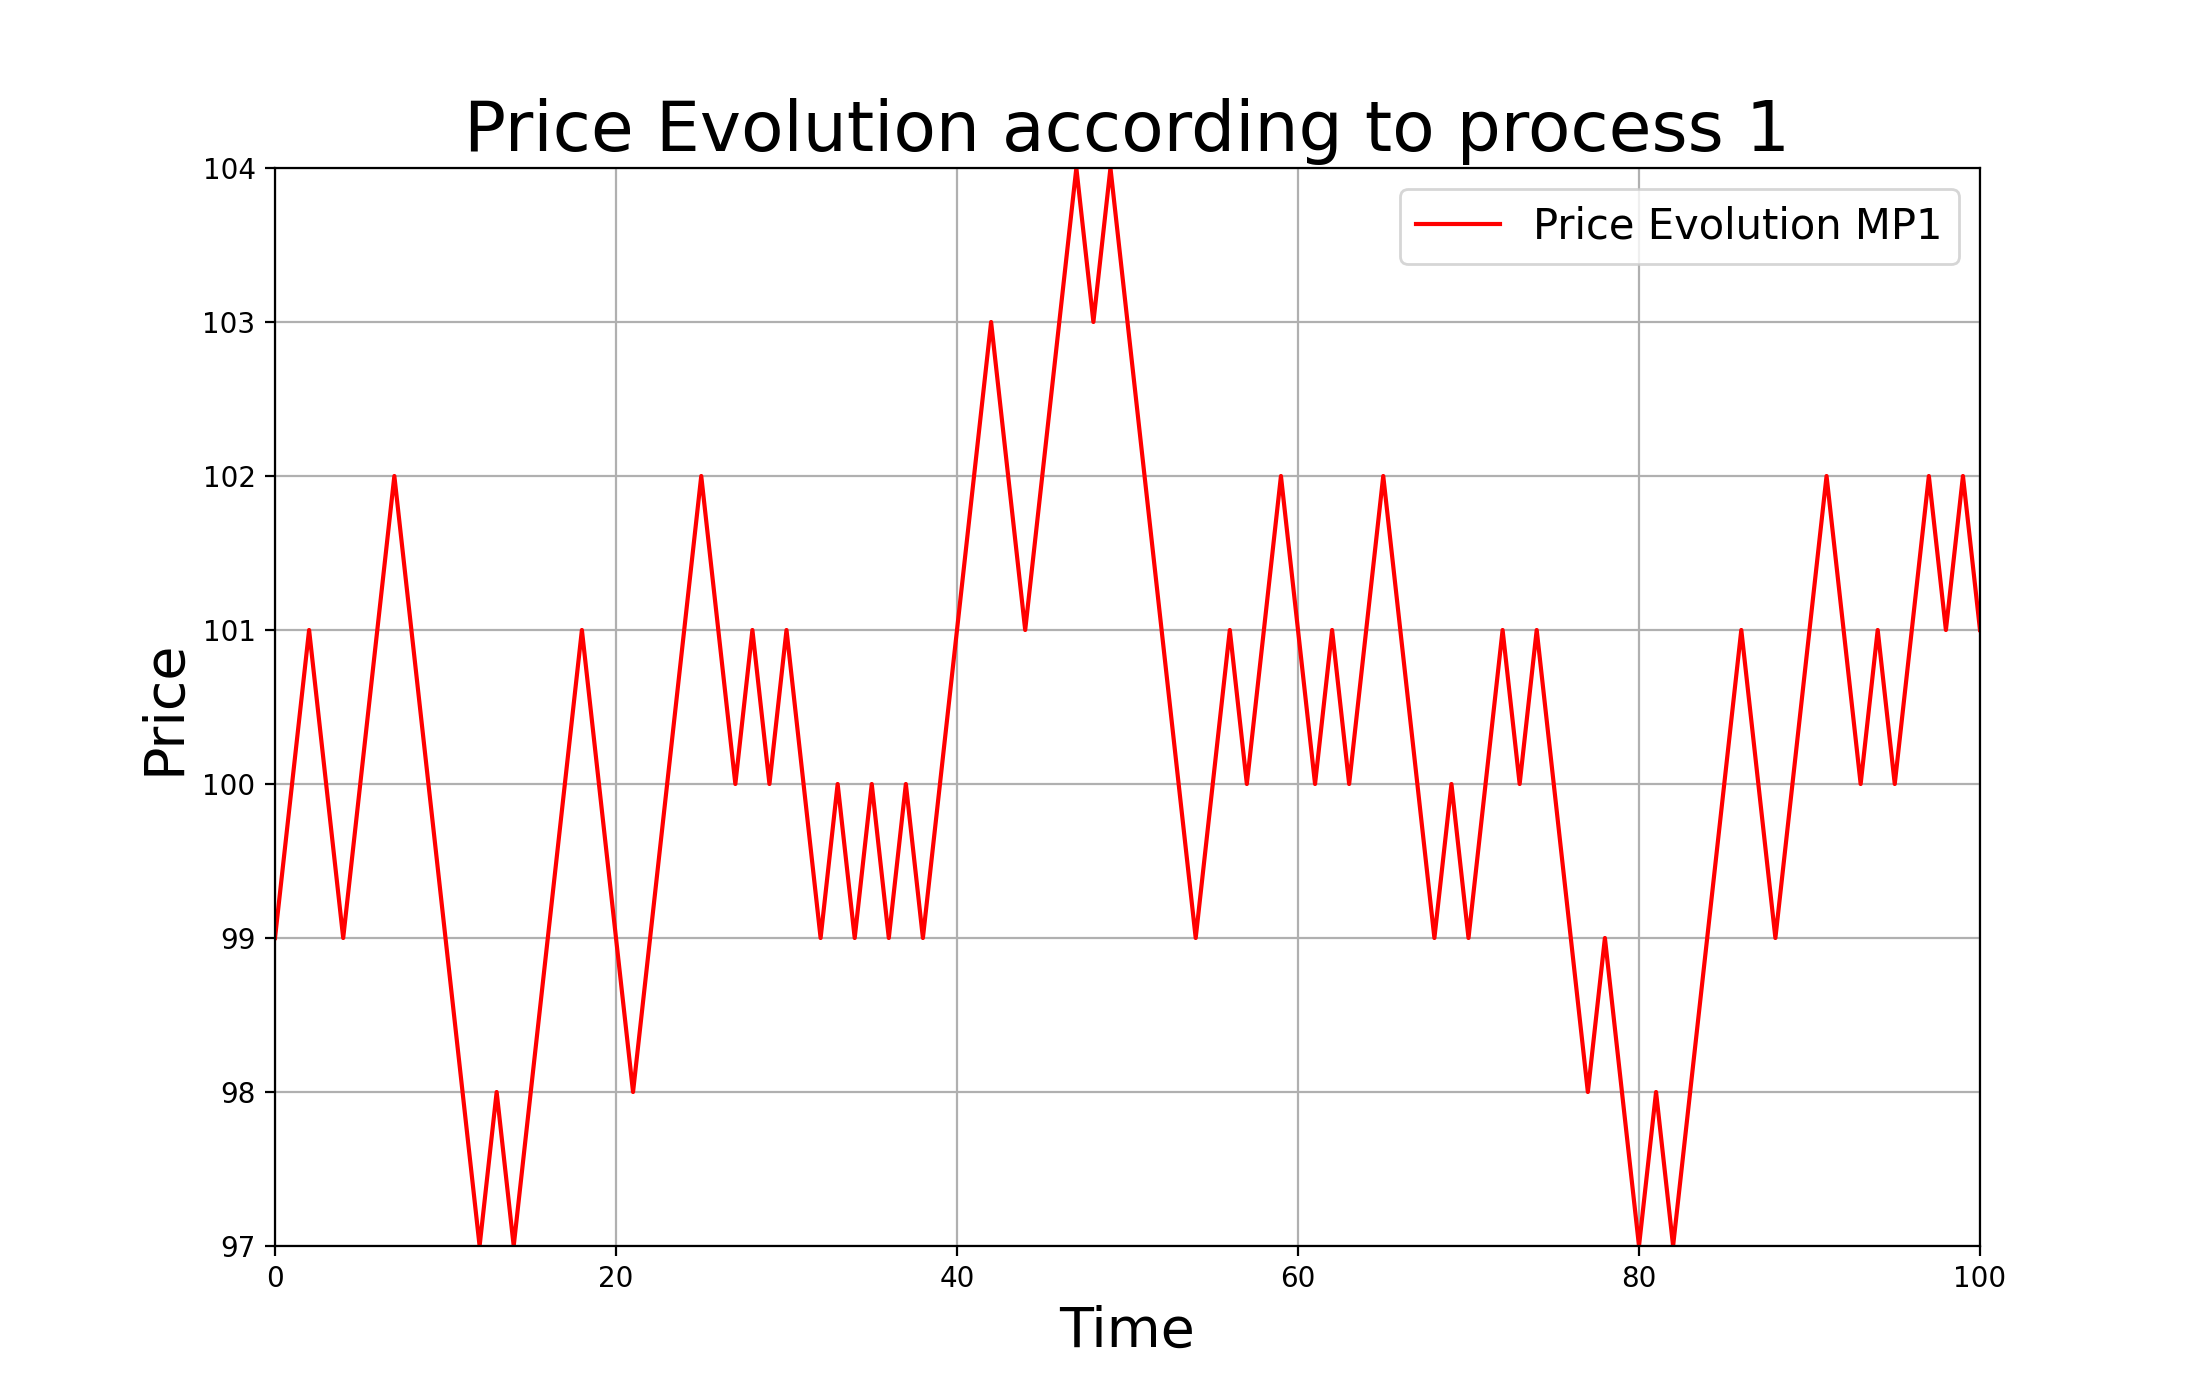
\includegraphics[width=\linewidth]{ex_price.png}
  \caption{Example Stock Price Process 1}
  \label{fig:rollDist}
\end{figure}

\begin{figure}
  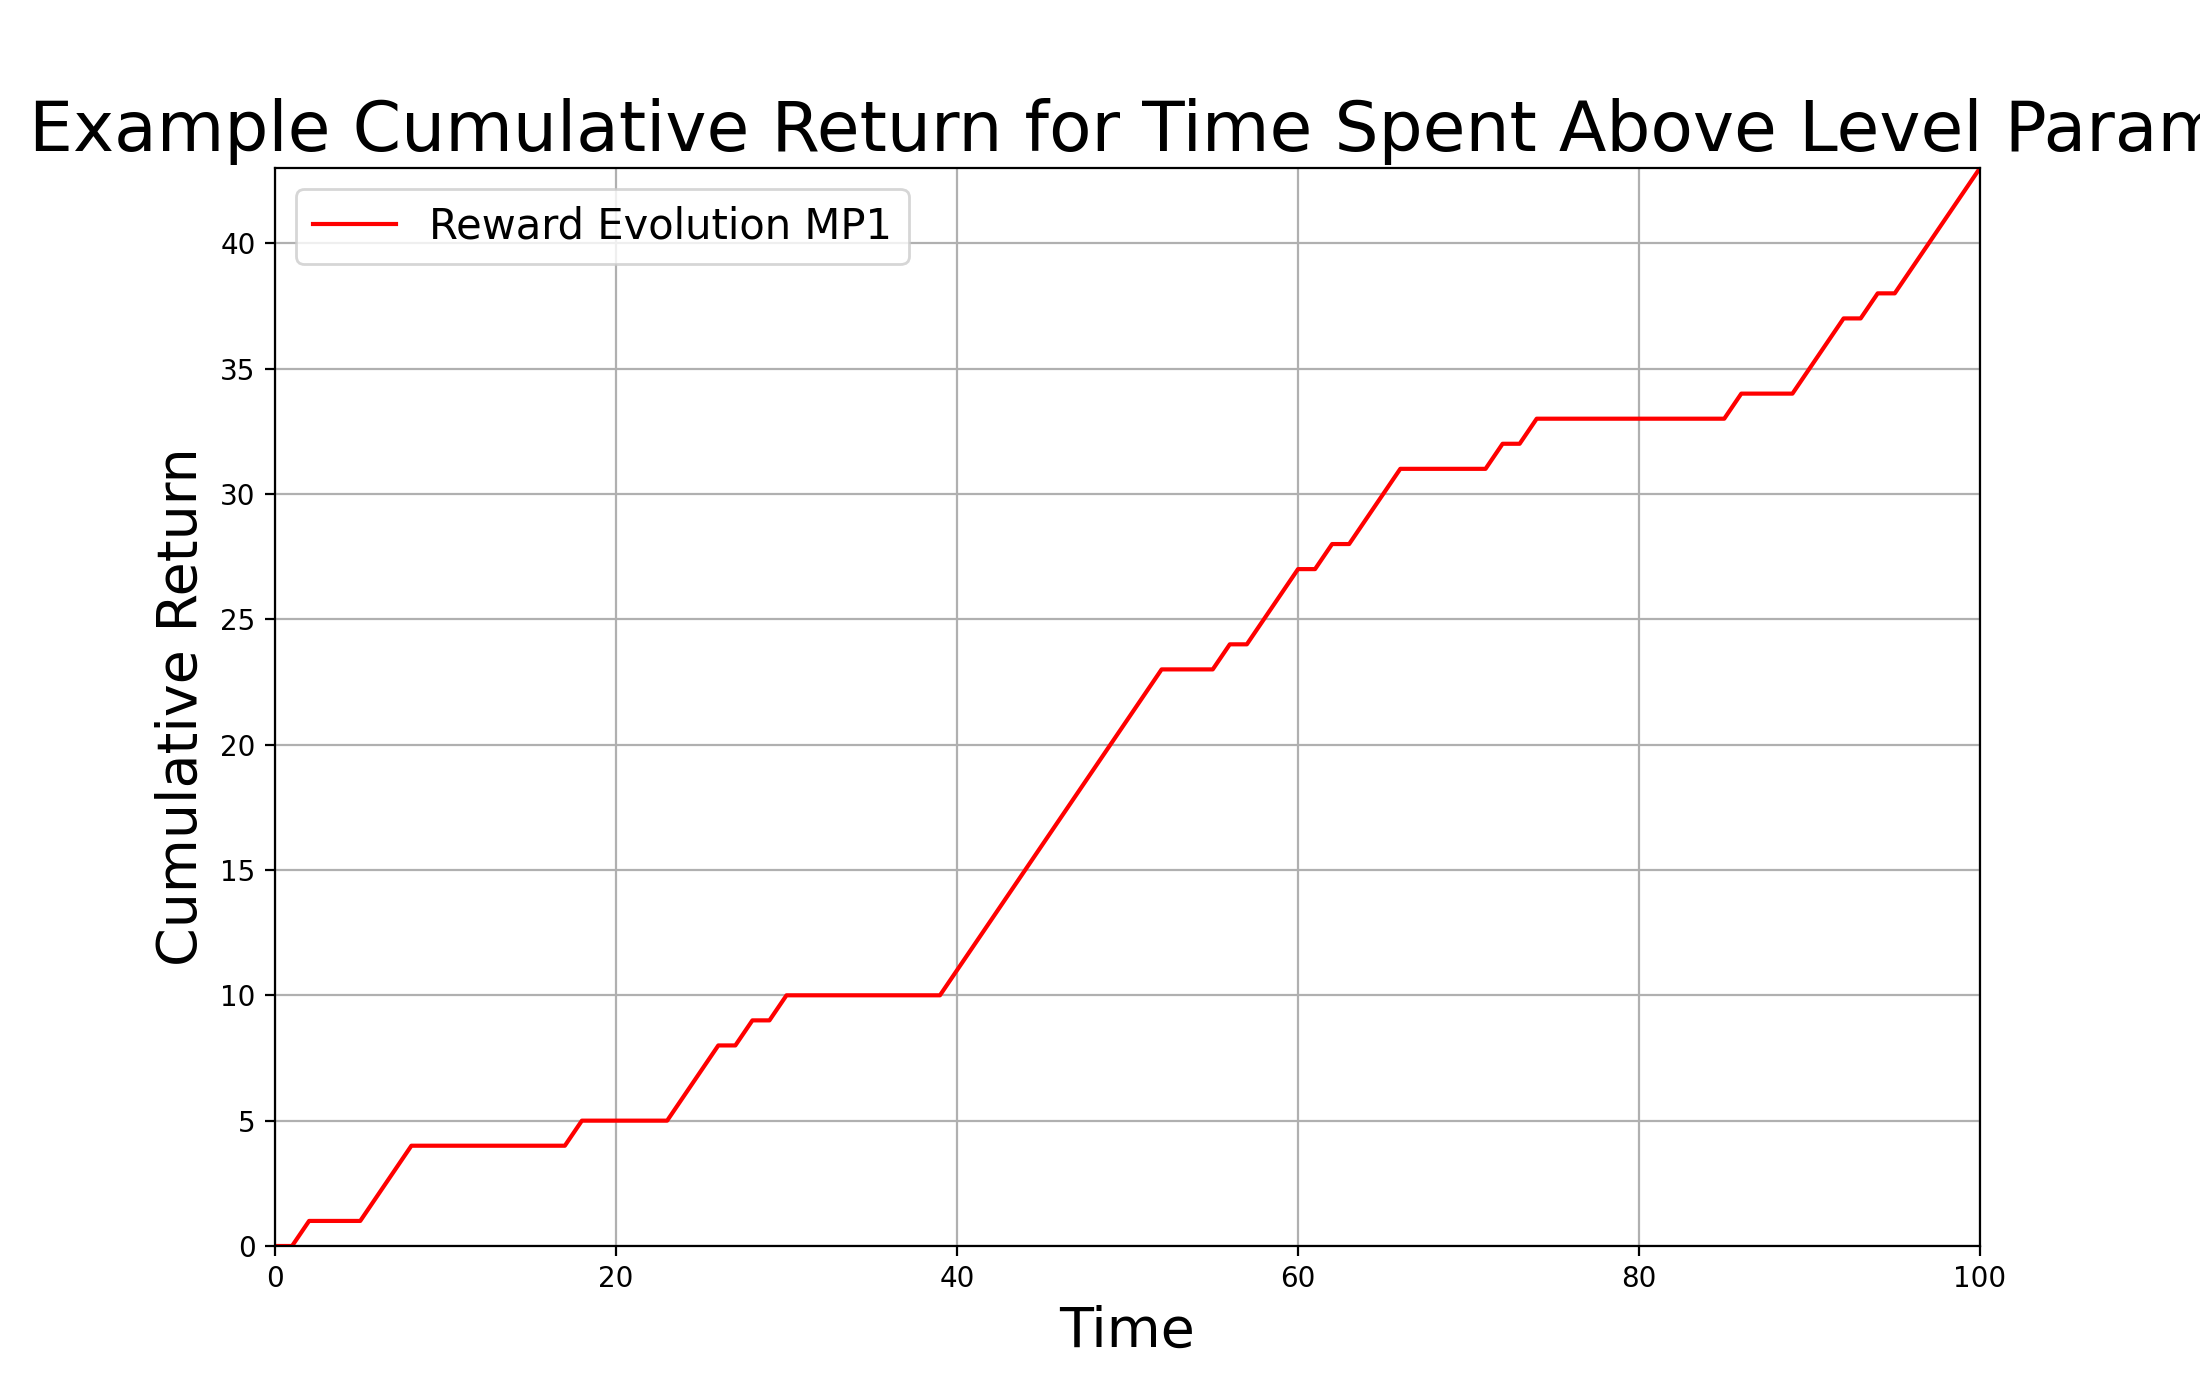
\includegraphics[width=\linewidth]{ex_rew.png}
  \caption{Example Return for customized Reward Function}
  \label{fig:term_out}
\end{figure}
\end{document}
